\section{Исследование парметров барьеров}

\subsection{Исследование ширины барьеров}
Ширина барьеров уменьшает вероятность прохождения электрона сквозь барьер и величину тока соответсвенно. 

Рассмотрим РТГС с шириной барьеров <<b>>:
\begin{enumerate}
	\item 10 монослоев;
	\item 7 монослоев;
	\item 5 монослоев;
	\item 3 монослоев.
\end{enumerate}

\subsubsection{Прозрачность РТГС}
\begin{figure}[h!]
	\centering
	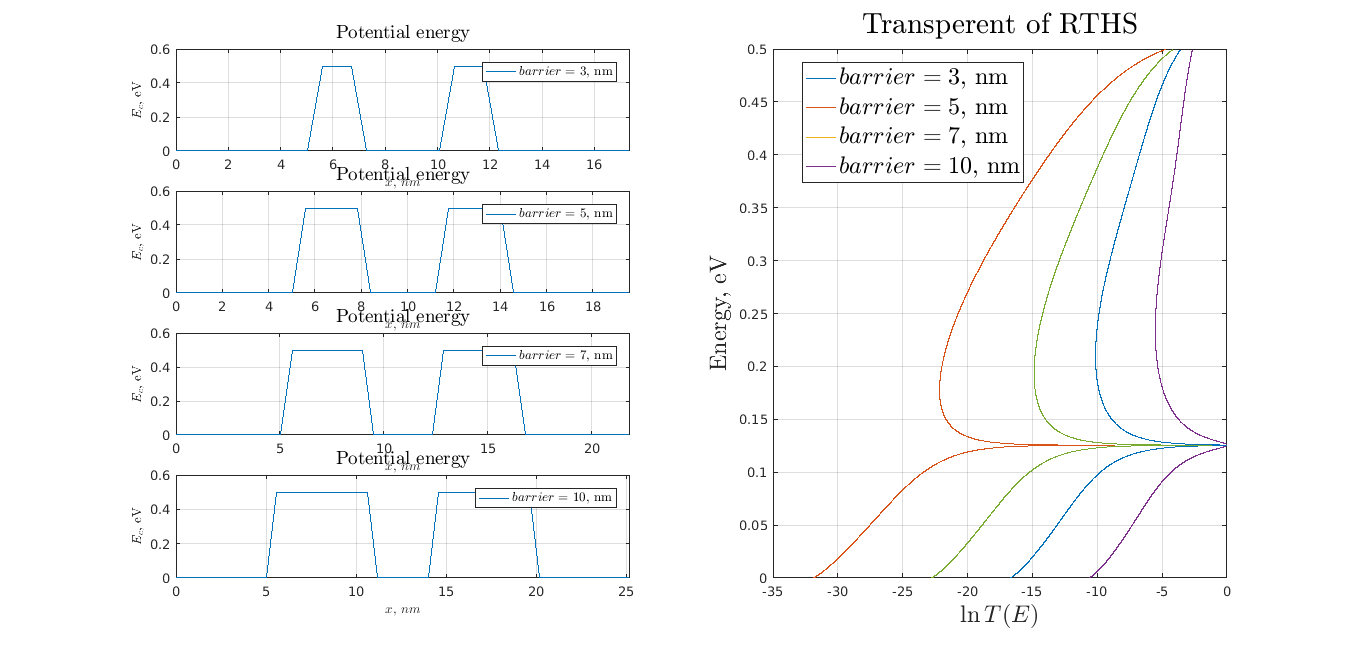
\includegraphics[width=\linewidth]{qbwt.png}
	\caption{Прозрачность РТГС при различных ширинах потенциальных барьеров}
	\label{fig:qbwt}
\end{figure}

Как видно на рис.~\ref{fig:qbwt} изменение ширины барьеров не сказывается на высоту резонансного уровня, а влияет только на прозрачность ГС. Увеличение ширины уменьшает прозрачность РТГС.

\subsubsection{ВАХ РТГС}
Пиковое значения тока изменяется значительно при изменении ширины потенциальных барьеров.
\begin{figure}[h!]
	\centering
	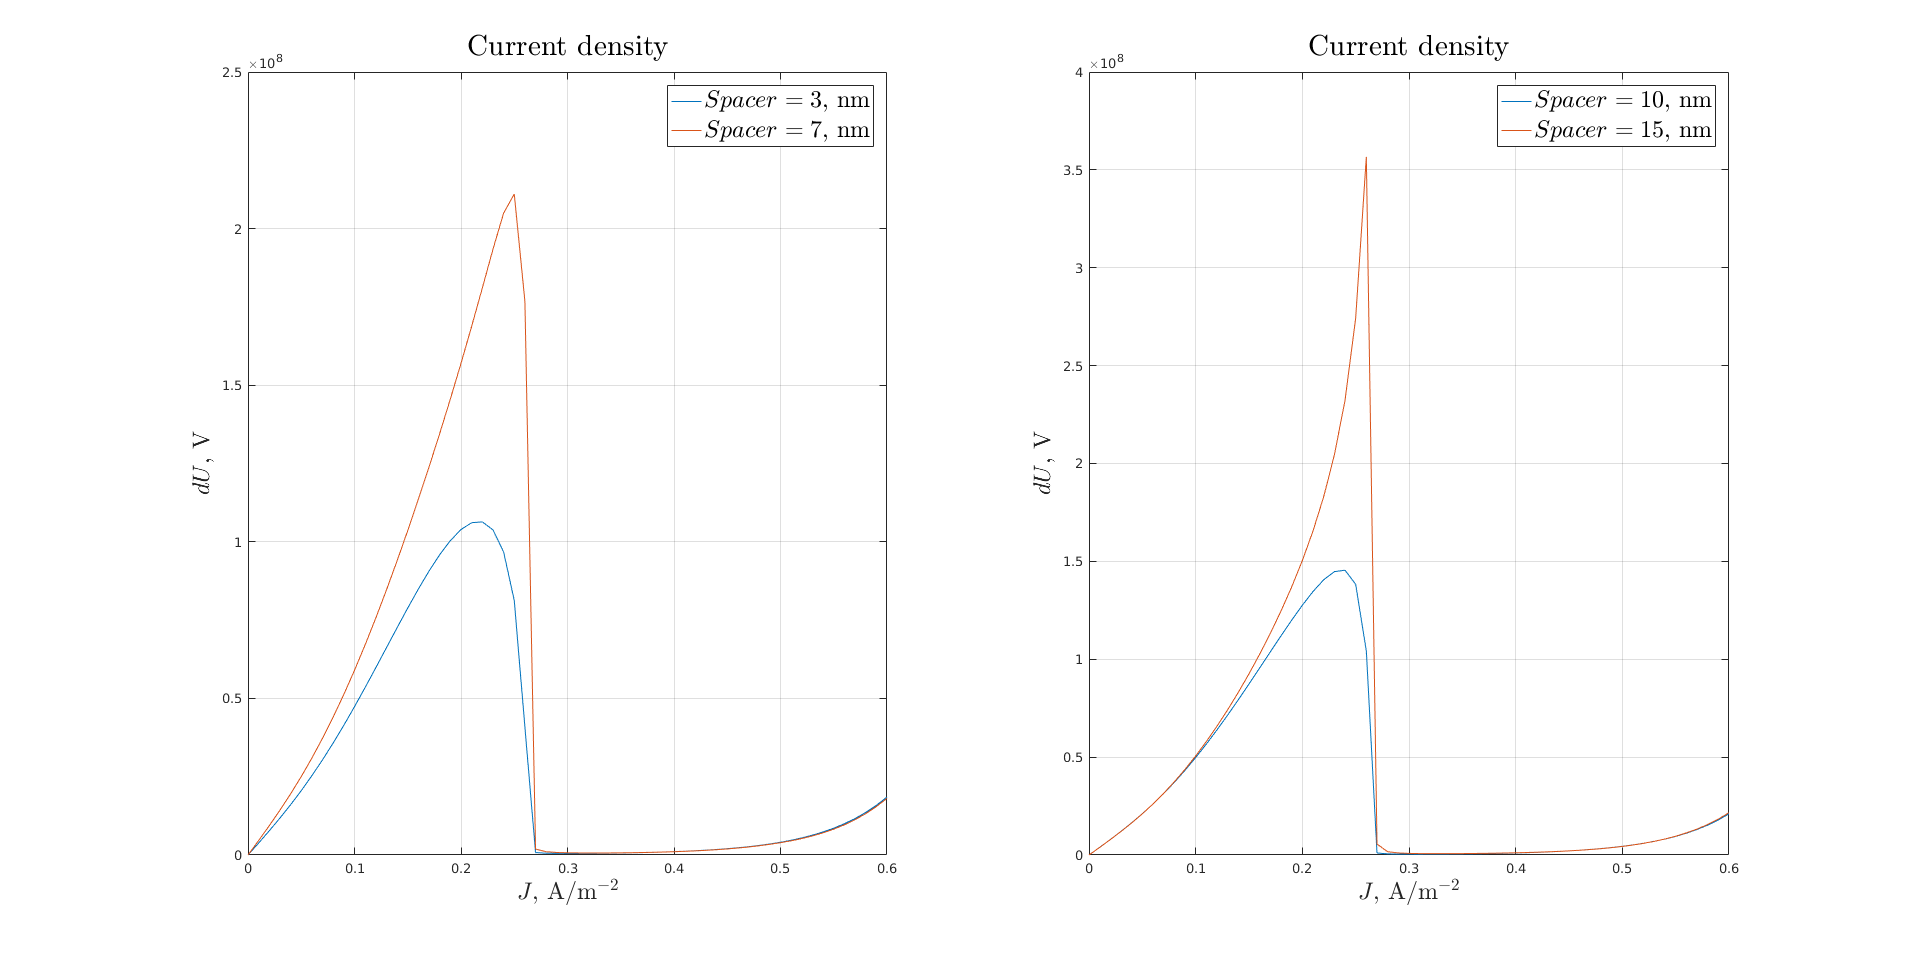
\includegraphics[width=\linewidth]{qbwj.png}
	\caption{Плотность тока через РТГС при различных ширинах потенциальных барьеров}
	\label{fig:qbwj}
\end{figure}

\subsection{Исследование высоты барьеров}
Рассмотрим высоту барьера:
\begin{enumerate}
	\item $1.0 eV$;
	\item $0.7 eV$;
	\item $0.5 eV$;
	\item $0.3 eV$.
\end{enumerate}

\subsubsection{Прозрачность РТГС}

В соответствии с рис.\ref{fig:qbht} с уменьшением высоты барьера резонансный уровень подымается, а прозрачность РТГС увеличивается.

\begin{figure}[h!]
	\centering
	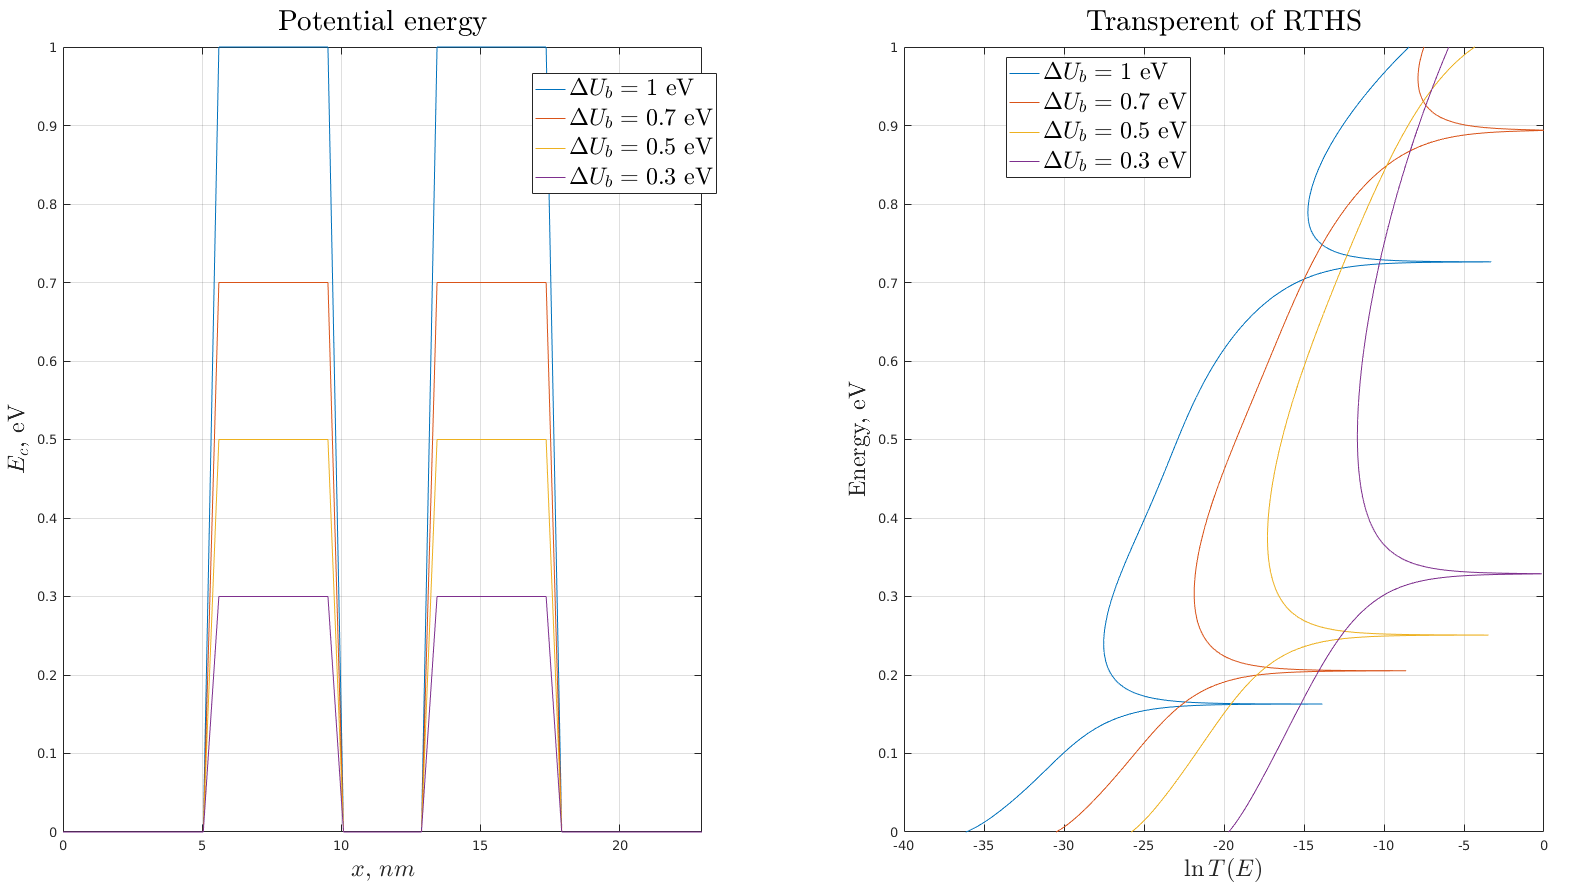
\includegraphics[width=0.7\linewidth]{qbht.png}
	\caption{Прозрачность РТГС при различных высотах потенциальных барьеров}
	\label{fig:qbht}
\end{figure}

\subsubsection{ВАХ РТГС}
Уменьшение высоты барьера повышает пиковое значение тока на порядок, при этом пиковое напряжение смещается незначительно.
\begin{figure}[h!]
	\centering
	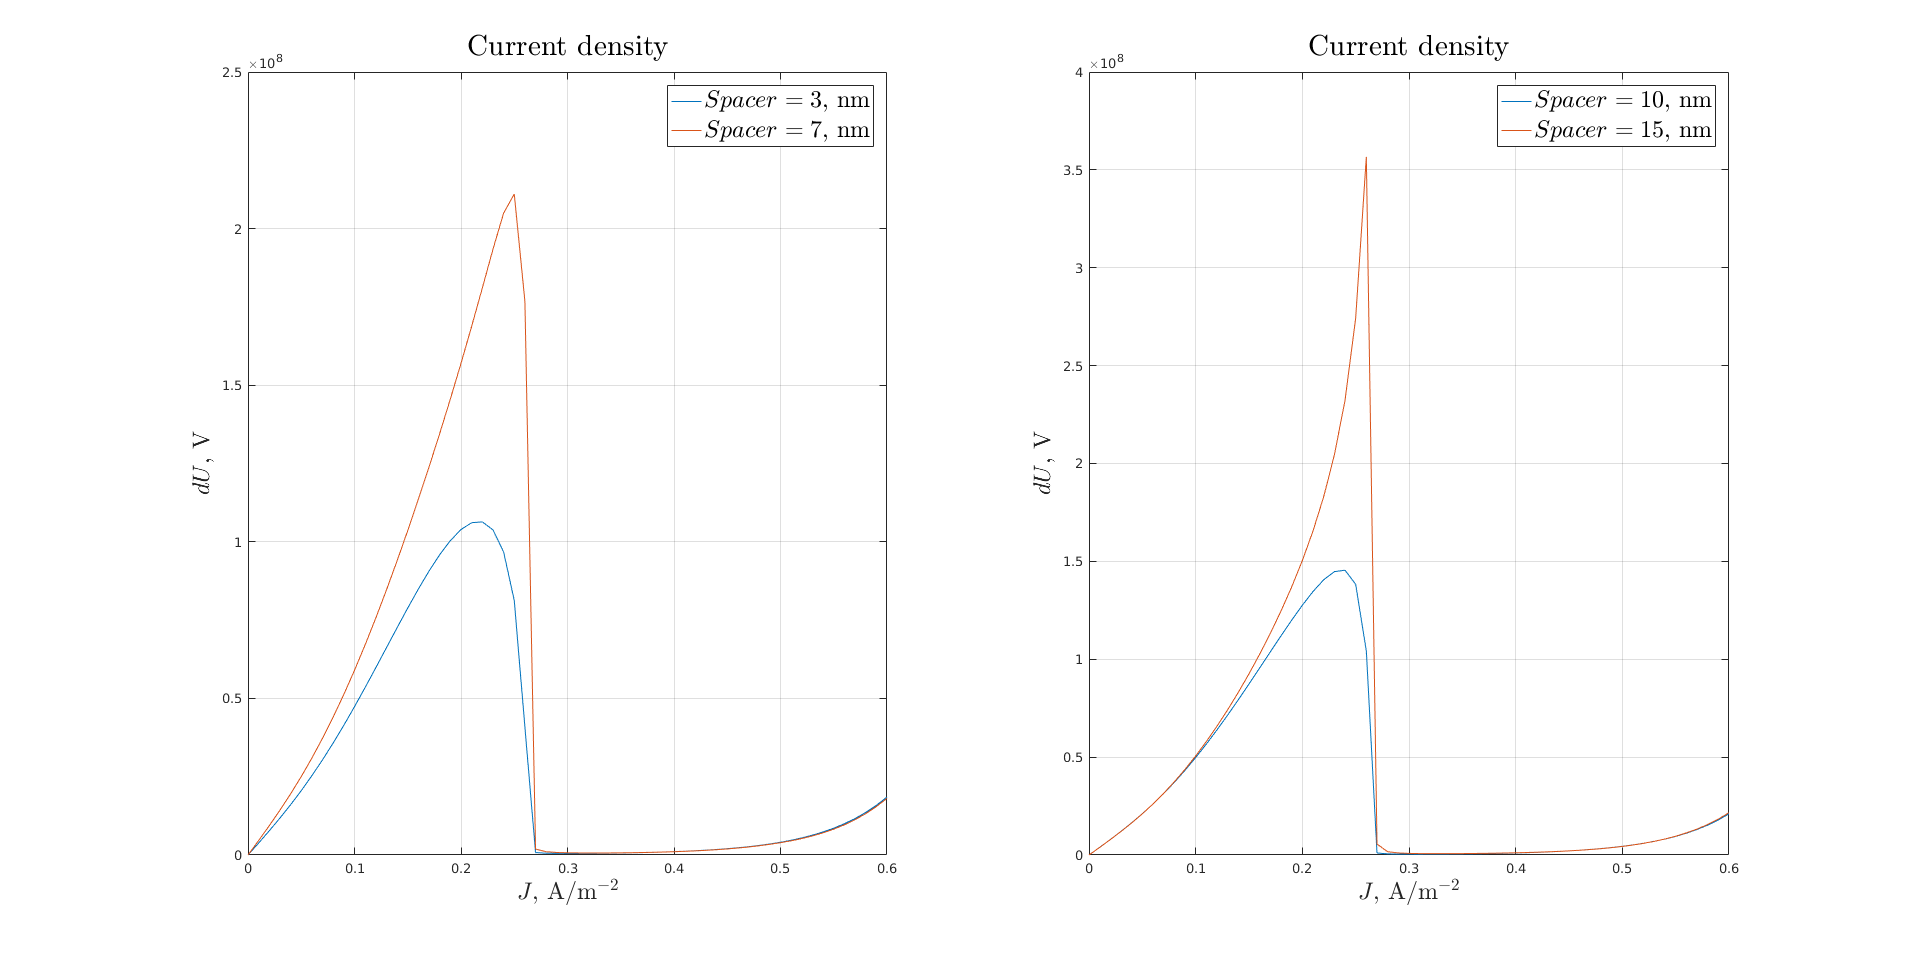
\includegraphics[width=0.7\linewidth]{qbwj.png}
	\caption{Плотность тока через РТГС при различных высотах потенциальных барьеров}
	\label{fig:qbwj}
\end{figure}

\subsection{Вывод}
Уменьшение ширины и высоты барьеров повышает вероятность туннелирования и тем самым увеличивает туннельную прозрачность исследуемой РГТС и плотность тока соответственно.
